\subsection{The non-locality of the real space operators} \label{sec:radial_locality}
%
\begin{figure}[t]
\centering
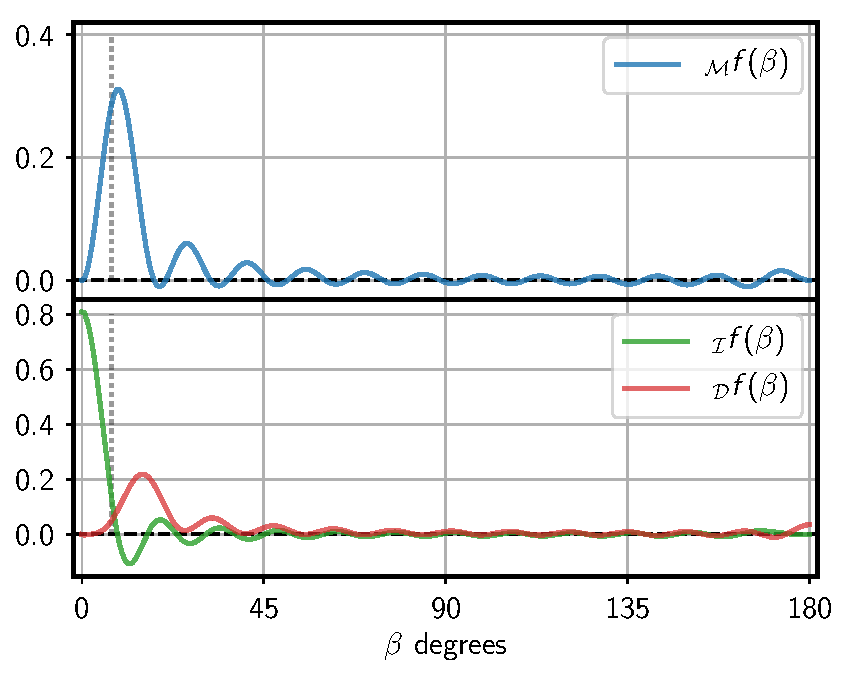
\includegraphics[width=0.8\columnwidth]{beta_kernel.pdf}
\caption{The figure depicts the radial part of the convolution kernels. These radial function have been evaluated with the band limit fixed at $\ell \in [2,24]$. The vertical dashed line marks the approximate Healpix pixel size of a NSIDE=8, which is the lowest resolution that allows access to $\ell_{\rm max}=24$.}
\label{fig:beta_kernel}
\end{figure}
%
Above, we have explored in detail the  azimuthal dependence of the real space kernels.  Here we probe the radial dependence, which both  determines the non-locality of the operators and encodes all their multipole dependencies. For illustration, \fig{fig:beta_kernel} shows the radial kernels ${_{\mm}f}, {_{\md}f},{_{\mi}f}$, evaluated using the respective multipole sums given in \eq{eq:rad_ker_queb} and \eq{eq:f2_rad_ker} in the band limit $\ell \in [2,24]$. We choose such a low band limit to highlight some key features of their radial profile.
%
\begin{figure}[t]
\subfigure[\label{fig:fbeta}]{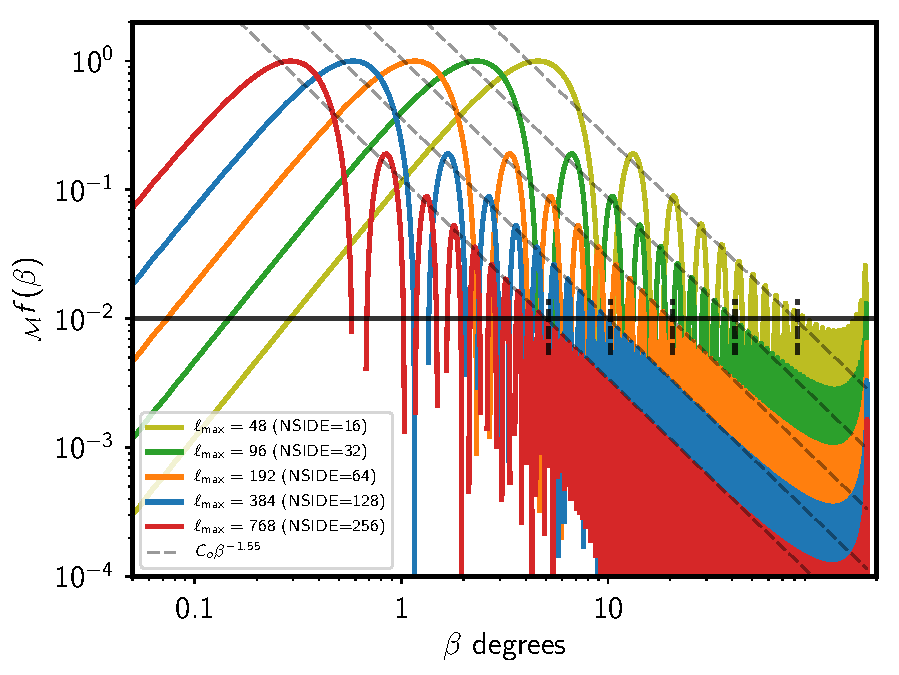
\includegraphics[width=0.325\columnwidth]{rad_ker_fn_of_ellmax.pdf}}\hfill
\subfigure[\label{fig:dfbeta}]{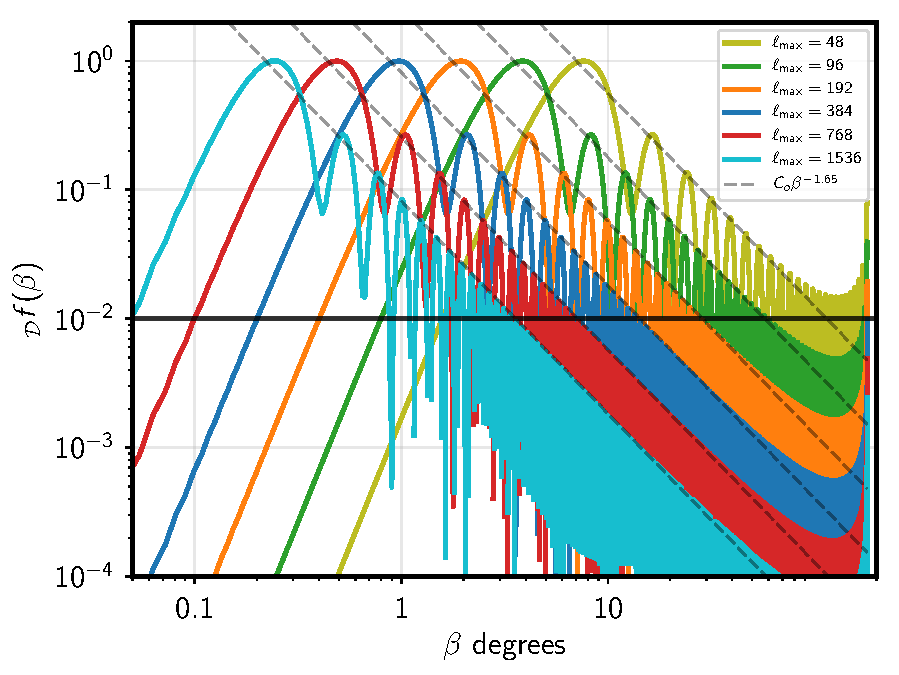
\includegraphics[width=0.325\columnwidth]{rad_ker_d_fn_of_ellmax.pdf}}\hfill
\subfigure[\label{fig:ifbeta}]{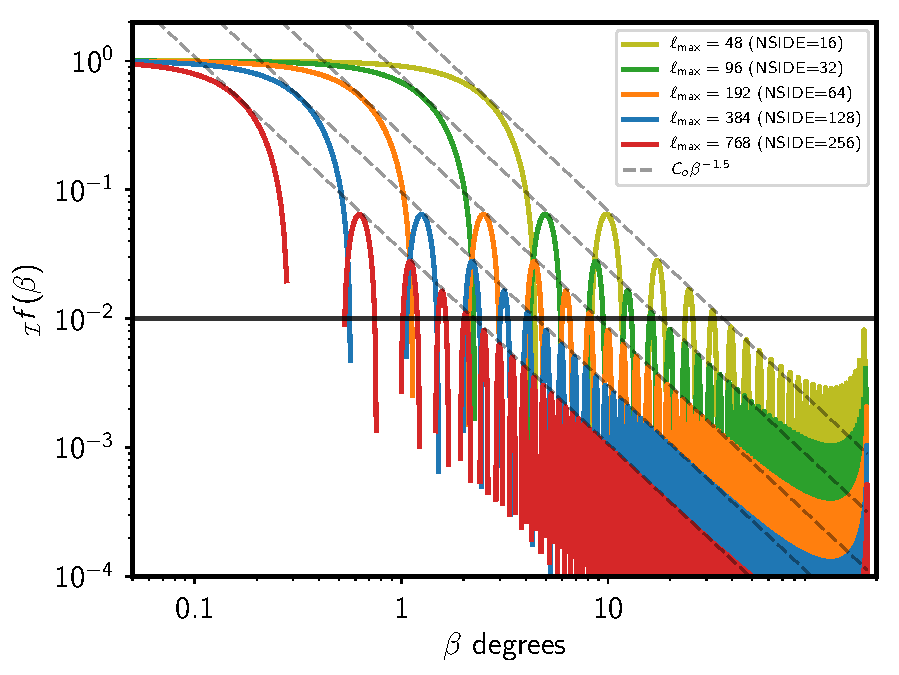
\includegraphics[width=0.325\columnwidth]{rad_ker_i_fn_of_ellmax.pdf}}\hfill
\centering
\subfigure[\label{fig:fbeta_avg}]{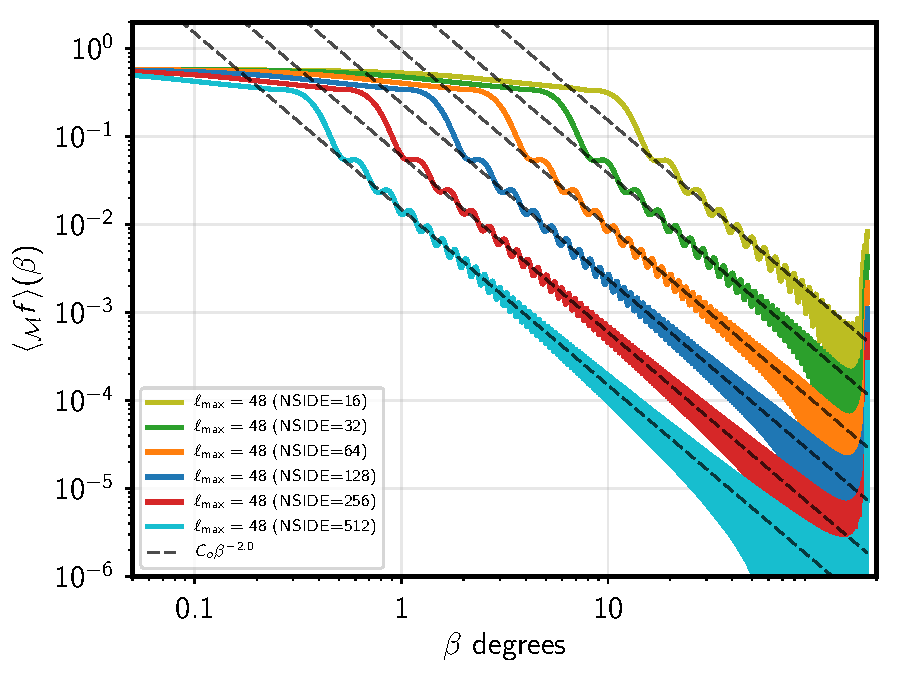
\includegraphics[width=0.325\columnwidth]{rad_ker_fn_of_ellmax_zaldariagga_scaling.pdf}}
\subfigure[\label{fig:dfbeta_avg}]{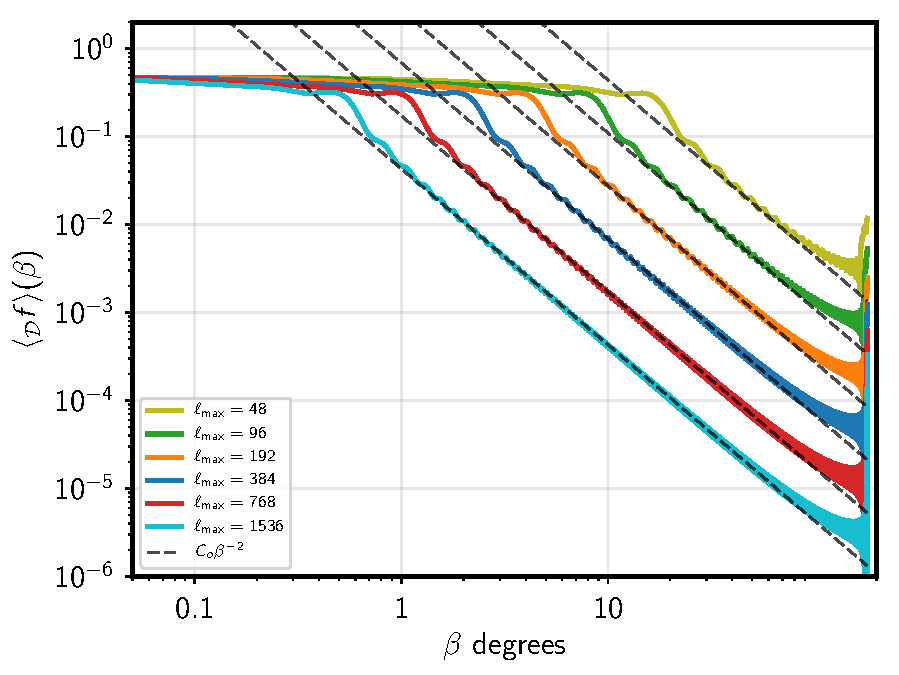
\includegraphics[width=0.325\columnwidth]{rad_ker_i_fn_of_ellmax_zaldariagga_scaling.pdf}}

\caption{This figures depicts the radial functions for the different kernels and varying band limit set by fixed $\ell_{\rm min}=2$ and varying $\ell_{\rm max}$ as indicated by their legends. \fig{fig:fbeta} depicts ${_{\mm}f}(\beta,\ell_{\rm min},\ell_{\rm max})$, \fig{fig:dfbeta} depicts ${}_{\md}f(\beta,\ell_{\rm min},\ell_{\rm max})$ and  \fig{fig:ifbeta} depicts ${}_{\mi}f(\beta,\ell_{\rm min},\ell_{\rm max})$ respectively. All the curves are normalized such that their maxima is set to unity. The horizontal solid black line marks the location where the amplitude of the respective kernels fall below 1\% of its maximum. The thin slanted dashed gray lines indicate a power law fit (by eye) to the envelope of the radial functions. The thick black short vertical dashed lines indicate the transition points as predicted by the empirically derived relation for the non-locality parameter $\beta_0={\rm min}(180^\circ,180^\circ \times 22/\ell_{\rm max})$. \fig{fig:fbeta_avg} and  \fig{fig:dfbeta_avg} depict the radial functions $\langle{_{\mm}f}(\beta,\ell_{\rm min},\ell_{\rm max})\rangle$ and $\langle{_{\md}f}(\beta,\ell_{\rm min},\ell_{\rm max})\rangle$ respectively where $\langle \cdots \rangle$ denotes a moving average over a step function centered at $\beta$ and has width $1.4\beta_0$. These smoothed functions are seen to be well fit by a power law $\propto \beta^{-2}$  and depict the average radial response.}
\label{fig:rad_ker_decay}
\end{figure}
%

The function ${_{\mm}f}$ is the radial part of the kernel that translates the Stokes parameters $Q$/$U$ to scalars $E$/$B$ and vice versa.  It has an oscillatory nature at intermediate angular separations and vanishes as $\beta \rightarrow 0$ and $\beta \rightarrow \pi$ (this is critical to ensure that the derived fields have the necessary spin properties), since the Euler angles $\alpha$, $\gamma$ are not uniquely defined at those separations.

The radial part of the kernel that decomposes the  Stokes parameters into parts that correspond to $E$ and $B$ modes  are also  necessarily non-local.  The function ${_{\mi}f}$ is the radial part of the band limited delta function $\mi$.  It expectedly has its maxima at $\beta=0$ and decays with increasing angular separation.  ${_{\md}f}$ has a vanishing value in the region where $\beta \rightarrow 0$ however it does not vanish at $\beta \rightarrow \pi$ as seen in \fig{fig:beta_kernel}.

\paragraph{Band limit dependence.} 
To quantify the non-locality of the real space operators, we study the radial extent of the respective radial kernels and their dependence on the maximum multipole accessible. We evaluate the radial functions for different values of $\ell_{\rm max}$, while keeping the lowest multipole fixed at $\ell_{\rm min}=2$. 

The resultant set of radial function are depicted in \fig{fig:rad_ker_decay}. The amplitude of these radial function scales up as $\propto \ell_{\rm max}^2$.  For clarity in the plot, their global maxima are normalized to unity.  This normalization highlights the key feature, that on increasing $\ell_{\rm max}$ the radial kernels shift left, attaining their global maxima at progressively small angular distances $\beta$.  At intermediate values of $\beta$, the envelope of the radial functions is fit well by a power law $ \propto \beta^{-n}$.  As the band limit changes, the small angle portion of the radial functions have a similar shape.

These finding are neatly summarized in the observation that the radial functions with different maximum multipoles are approximately self-similar over many oscillations, and are related by this telescoping and scaling property:
\begin{equation}{}_rf(\beta,2,\ell_{\rm max}) \approx \Big[\frac{\ell_{\rm max}}{\ell'_{\rm max}}\Big]^2{}_rf(\beta'=\frac{\ell'_{\rm max}}{\ell_{\rm max}} \beta ,2,\ell'_{\rm max}),\end{equation}
where ${}_rf , r \in [\mm, \md,\mi]$ denotes all the different radial functions. This telescoping property encapsulates both the amplitude scaling and leftward shift of the radial kernels on increasing the maximum multipole. {Specifically, when $\ell_{\rm max} > \ell'_{\rm max}$, the global maxima of the kernel with maximum multipole $\ell_{\rm max}$ is amplified by a factor $(\ell_{\rm max}/\ell'_{\rm max})^2$ with respect to the kernel defined by the maximum multipole $\ell'_{\rm max}$, while the period of the oscillation is compressed by a factor $(\ell'_{\rm max}/\ell_{\rm max})$. The detailed accuracy of this approximation varies with the angular separation $\beta$ and the difference in the maximum multipoles ($\ell_{\rm max}$, $\ell'_{\rm max}$)  used in evaluating the two functions.}

To quantify the non-locality of the scalar modes $E/B$, we can define a characteristic angular radius of the region from which the kernels get most of their contribution.   We define a non-locality parameter $\beta_{0}$ as the angular distance beyond which the function ${_{\mm}f}(\beta,\ell_{\rm min}=2,\ell_{\rm max})$ transitions to being consistently below 1\% of its maximum.
The empirical relation:
\beq
\beta_0= {\rm min}\left(180^\circ,180^\circ \frac{\ell_{0}}{\ell_{\rm max}} \right) \,,
\eeq
with $\ell_{0}=22$ provides a reasonable estimate of this transition point for ${}_{\mm}f$ as seen in \fig{fig:rad_ker_decay}. Setting $\ell_{0}=10$ and $\ell_{0}=32$ predicts the transition points for the functions ${}_{\mi}f$ and  ${}_{\md}f$ respectively.

The radial function ${}_\mm f(\beta)$ is oscillatory, regardless of the maximum $\ell_{\rm max}$. The envelope of the oscillation decays with angular separation at intermediate $\beta$ but increases as $\beta \rightarrow \pi$.  We find that the positive envelope of ${}_{\mm}f$ scales as $\beta^{-1.6}$ at intermediate $\beta$.  However, when we average over several oscillations with a moving window, we find that the average behavior at intermediate $\beta$ scales as $\beta^{-2}$, visible in \fig{fig:fbeta_avg}. We set the width of the smoothing window to $0.3\beta_0$, and this results in the narrowing of the smoothing width as the band limit increases, so as to keep the number of oscillations averaged over roughly the same.  This agrees with the hypothesis for the {flat sky and continuum case}, for which e.g. Zaldarriaga (2001) \cite{Zaldarriaga2001a} argued that form of the radial function has to be ${}_\mm f(\beta>0)\simeq\beta^{-2}$ to ensure that the Fourier modes of Stokes $Q/U$ relate to those of $E/B$ merely by rotations (with no scale dependence). In addition, we find that ${}_{\md}f$ under a moving average shows a similar scaling of $\beta^{-2}$, as seen in \fig{fig:dfbeta_avg}.
Applying a moving average on radial functions with increasing band limit, we see that a larger fraction of angular domain matches the scaling of $\beta^{-2}$.   Extrapolating this trend to the case of a very high band limit one expects this behavior to approach $\beta^{-2}$ across the domain $\beta\in[\epsilon,\pi-\epsilon]$ for $\epsilon \ll 1$. In essence the moving average can be understood as the averaging resulting from discrete sampling of a continuum field (one with an infinite band limit) where the width of the averaging window corresponds to the size of the pixel.

Near the edges of the domain $\beta \rightarrow 0,\pi$ the window function partly falls outside the domain and this is in part responsible for the scaling deviating from the power law, but it is also important to note that ${}_{\mm}f$ and ${}_{\md}f$ need to vanish at $\beta=0$ and therefore the sliding average in the vicinity of these points cannot have the same power law behavior.
